\section{High-Level Architecture}
The system follows a \textbf{client--server} pattern with a document database:
\begin{itemize}
  \item \textbf{Client:} React (Vite), Tailwind CSS, ShadCN-style components, React Router, React Hook Form + Zod, Axios (withCredentials), Zustand, Recharts.
  \item \textbf{Server:} Node.js, Express.js, Mongoose, Passport (Google), JWT, bcrypt, Helmet, CORS, Morgan, cookie-parser.
  \item \textbf{Database:} MongoDB collections for users, employees, tasks, performance records, alerts, application settings.
\end{itemize}

\begin{figure}[H]
  \centering
  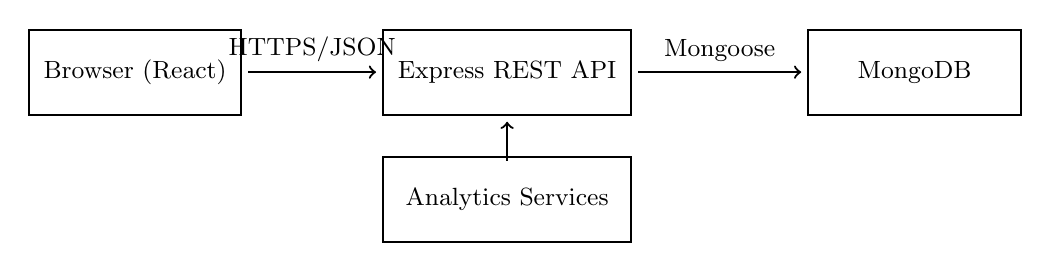
\begin{tikzpicture}[scale=0.9, every node/.style={font=\small}]
    \draw[thick] (0,0) rectangle (3,1.2) node[midway] {Browser (React)};
    \draw[thick] (5,0) rectangle (8.5,1.2) node[midway] {Express REST API};
    \draw[thick] (11,0) rectangle (14,1.2) node[midway] {MongoDB};
    \draw[->, thick] (3.1,0.6) -- node[above] {HTTPS/JSON} (4.9,0.6);
    \draw[->, thick] (8.6,0.6) -- node[above] {Mongoose} (10.9,0.6);
    \draw[thick] (5,-1.8) rectangle (8.5,-0.6) node[midway] {Analytics Services};
    \draw[->, thick] (6.75,-0.65) -- (6.75,-0.1);
  \end{tikzpicture}
  \caption{Logical deployment view (conceptual).}
  \label{fig:arch}
\end{figure}

\section{Data Model (Summary)}
Key entities:
\begin{itemize}
  \item \textbf{User:} identity, credential or Google id, role (\texttt{admin}|\texttt{manager}|\texttt{employee}).
  \item \textbf{Employee:} HR profile, skill tags, operational metrics, embedded performance history snapshots, cached attrition/promotion fields.
  \item \textbf{Task:} specification, required skills, lifecycle status, single assignee reference.
  \item \textbf{PerformanceRecord:} dimensional scores, weighted aggregate, embedded breakdown and explanation.
  \item \textbf{Alert:} typed message with severity and read flag.
  \item \textbf{AppSettings:} global performance weights.
\end{itemize}

\section{Control Flow --- Authentication}
Registration/login validates input, hashes passwords, signs JWT with server secret, sets HTTP-only cookie, and exposes \texttt{/api/auth/me} for session bootstrap. Google OAuth redirects through Passport; on success the same cookie issuance path executes.

\section{Control Flow --- Analytics}
Controllers delegate to \textbf{service modules}: performance engine, task allocation, attrition, anomaly, promotion. Services return JSON including \texttt{explanation} and/or \texttt{method} fields for UI and reporting. This separation keeps routes thin and enables unit-style reasoning about formulas.

\section{API Design}
RESTful resources under \texttt{/api/}: \texttt{auth}, \texttt{employees}, \texttt{tasks} (including \texttt{assign} and \texttt{recommend}), \texttt{performance}, \texttt{ml} (attrition, anomaly, promotion, task-match), \texttt{alerts}, \texttt{settings}. Errors return JSON with clear messages; validation failures list field issues.

\section{Security Design}
Role checks applied after authentication middleware. Employees are scoped to linked profiles for self-service routes. CORS restricted to configured client origin with credentials enabled. Passwords never returned from API; JWT not exposed to JavaScript when using HTTP-only cookies.
